\subsection{Multi-process coordination costs}
\label{eval:perf:multi-proc}

The most expensive system calls occur when {\tt libLinux} inadvertently duplicates work
with the host kernel.  
For instance, many of the file path and handle management calls duplicate some of the effort of the host file system,
leading to a 1--3\x{} slower implementation than native.
As the worst example,
{\tt fork+exit} is 5.9\x{} slower than Linux.
Profiling indicates that about one sixth of this overhead is in process creation, which 
takes additional work to create a clean \picoproc{} on Linux; we expect this overhead could be reduced
with a kernel-level implementation of the process creation ABI, rather than emulating this behavior on {\tt clone}.
Another half of the overhead comes from the
{\tt libLinux} checkpointing code (commensurate with the data in Table~\ref{tab:graphene:lmbench}), which 
includes a substantial amount of serialization effort which might be reduced by checkpointing the data structures in place.
A more competitive {\tt fork} will require host support and additional {\tt libLinux} tuning.
%Thus, we think a competitive {\tt fork} implementation will require both a more suitable host kernel
%and more tuning in the {\tt libLinux} code. 
%\fixmewkj{explain why TCP faster than UDP?}


\fixme{talk about a limitation of improving fork. check this.}
One way to further optimize \syscall{fork} is to reduce or avoid enclave creation time; one can potentially pre-launch a child enclave, and then migrate the process contents later when \syscall{fork} is called.
There might be another opportunity to improve the latency of process migration,
if copy-on-write sharing of enclave pages can be supported in future generations of SGX.
%Unfortunately, sending the process contents is difficult to avoid in \syscall{fork},
%as SGX disallows sharing enclave memory between multiple enclaves.

%\fixmedp{I assume 5.4 isn't done yet}


%Adding more detail of KVM environment
%Unless otherwise noted, \graphenesgx{} measurements include the Phosphor instrumentation.


\begin{table}[t!b!]
\footnotesize
\centering
\bgroup
\def\arraystretch{1.1}
\setlength{\tabcolsep}{.5em}
\begin{tabular}{|l|>{\palign{r}}p{3em}r|>{\palign{r}}p{3em}rr|>{\palign{r}}p{3em}rr|>{\palign{r}}p{4em}rr|}
\hline
&\multicolumn{11}{c|}{System call latency (\usec{}), +/- Confidence Interval, \% Overhead} \\
\hline
\multicolumn{1}{|c|}{{\bf Test}} &
\multicolumn{2}{c|}{{\bf Linux \linuxversion{}}} &
\multicolumn{3}{c|}{{\bf \graphene{}}} & \multicolumn{3}{c|}{{\bf \graphene{}+SC+RM}} & \multicolumn{3}{c|}{{\bf \graphenesgx{}}} \\
&
\usec{} & +/- & 
\usec{} & +/- & \%O &
\usec{} & +/- & \%O &
s & +/- & O \\
\hline

fork/exit	&	193	&	6	&	1,004	&	22	&	421	&	1,050	&	25	&	444	&	1.227	s &	.069	s &	6,360	$\times$	 \\\hline
double fork/exit	&	562	&	18	&	2,241	&	74	&	299	&	2,325	&	28	&	314	&	2.423	s &	.086	s &	4,314	$\times$	 \\\hline
vfork/exit	&	456	&	10	&	1,305	&	288	&	186	&	1,352	&	239	&	197	&	1.156	s &	.056	s &	2,536	$\times$	 \\\hline
fork/execve	&	610	&	28	&	1,470	&	12	&	141	&	1,570	&	14	&	158	&	1.282	s &	.067	s &	2,102	$\times$	 \\\hline
double fork/execve	&	979	&	23	&	2,837	&	176	&	190	&	2,932	&	63	&	199	&	2.311	s &	.107	s &	2,359	$\times$	 \\\hline
%fork/dash	&	1,491	&	5	&	3,593	&	156	&	141	&	3,738	&	27	&	151	&		s &		s &	-1	$\times$	 \\\hline

\end{tabular}
\egroup
\caption{Benchmark results of various combinations of \syscall{fork}, \syscall{vfork}, and \syscall{execve}, based on \lmbench{} 2.5. Comparison is among (1) native Linux processes, (2) \graphene{} \picoprocs{} on Linux host, both without and with JIT-optimized SECCOMP filter ({\bf +SC}) and reference monitor ({\bf +RM}), and (3) \graphene{} in SGX enclaves.
Latency is in microseconds, except for \graphenesgx{}, which is orders-of-magnitude slower. Lower latency is better.
Overheads are relative to Linux \linuxversion{}; negative overheads indicate improved performance.} 
\label{tab:eval:lmbench-fork}
\end{table}







Figure~\ref{fig:eval:sgx-fork}(c) shows the overhead of forking a process.
As described in Section~\ref{sec:sgx:shield:multiproc}, the latency of \syscall{fork} in \graphenesgx{} is affected by three factors:
creation of a new enclave, local attestation of the integrity, and duplicating the process state over an encrypted RPC stream.
Combining these factors, \syscall{fork} is one of the most expensive calls in \graphenesgx{}.
%, but at least it is supported natively on the current hardware.
The default enclave size is 256MB.
%which takes \roughly{}0.5s to create. 
Our evaluation shows that the latency of forking a process is around 0.8s (16MB process) to 2.7s (128MB process), but can be more expensive if the parent process uses more memory.
The trend matches the performance of \graphene{} without the bulk IPC optimization.
\fixmedp{If you want, some thoughts on how this might be improved in the future would be nice...  One good suggestion is recycling enclaves, or pre-forking so measurements can be done in parallel}
%Due to the overhead on \funcname{fork}, \graphenesgx{} is not suitable for fork-intensive workloads like Bash scripts
%if performance is critical.


\begin{figure*}[t!]
\centering
\begin{minipage}{.45\textwidth}
\centering
\footnotesize
\vspace{6pt}
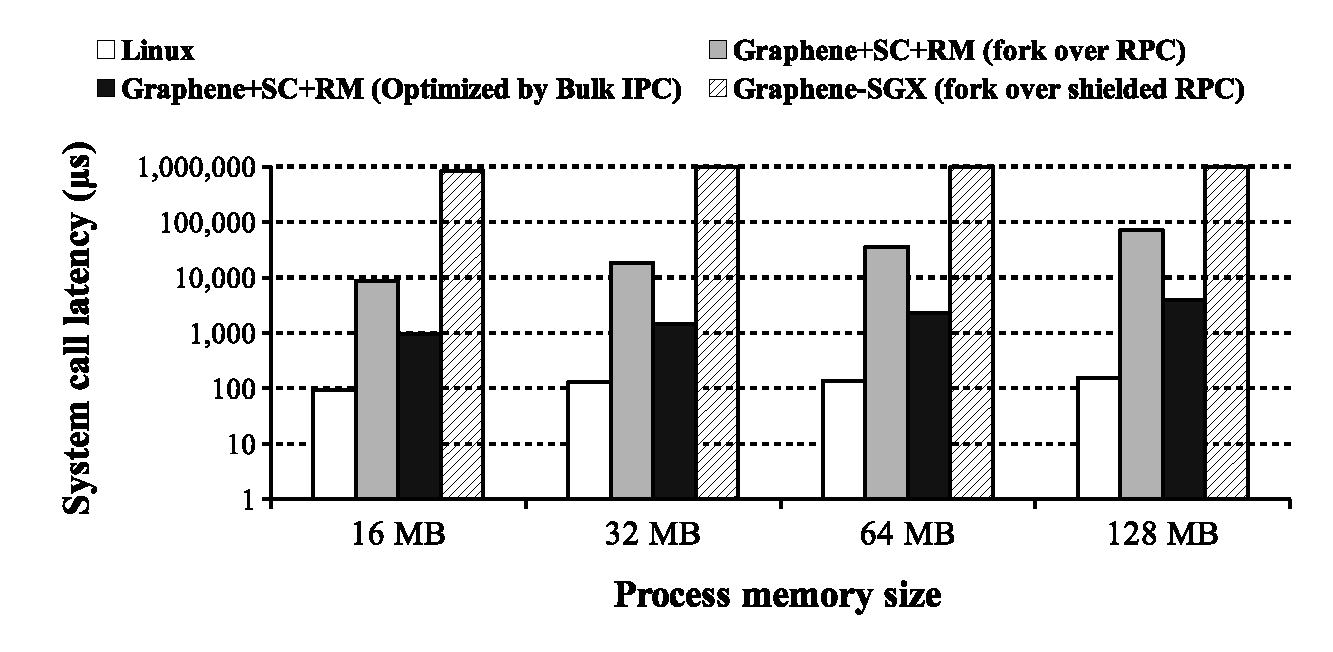
\includegraphics[width=\linewidth]{sgx/fork-latency}\\
\vspace{3pt}
{\bf (c) Fork a process}
\vspace{6pt}
\end{minipage}
\caption{Latency of some expensive system calls in \graphenesgx{}, including opening and reading a secured (authenticated) file, and forking a new process. The results are compared with native Linux and \graphene{}.}
\label{fig:eval:sgx-fork}
\end{figure*}







We also measure the overhead of isolating a \graphene{} \picoproc{} inside the reference monitor.
Because most filtering rules can be statically loaded into the kernel,
the cost of filtering is negligible with few exceptions.
%TCP and UDP latency is increased slightly because the monitor checks
%the arguments of the {\tt connect} system call.
Only calls that
involve path traversals, such as {\tt open} and {\tt exec}, result in substantial overheads relative to \graphene{}.
%%, adding an additional 100--200\% overhead. This is 
%because the AppArmor extensions must verify that
%the requested paths are in the permitted file system view.
%Alternative implementations, such as a {\tt chroot-ed} environment using the aufs unioning file system version 3.0~\cite{aufs},
%resulted in opens that were {\em twice} as slow as our LSM extensions.
An efficient implementation of an environment similar to FreeBSD  jails~\cite{jails}
would make all reference monitoring overheads negligible.

\begin{table}[t!b!]
\footnotesize
\centering
\begin{tabular}{|ll|rr|rrr|}
\hline
\multicolumn{2}{|c|}{{\bf Test}} &
\multicolumn{2}{c|}{{\bf Linux}} &
\multicolumn{3}{c|}{{\bf \graphene{}}} \\
& & \us{} & +/- & \us{} & +/- & \\
\hline
msgget   & in-process    & 3320	& 0.7 &  2823 & 0.3 &	-15	\%		\\
(create) & inter-process & 3336	& 0.5 &  2879 & 3.6 &	-14	\%		\\
& persistent    &  N/A	&     & 10015 & 0.7 &	202	\%      \\
\hline								
msgget   & in-process    & 3245	& 0.5 &   137 & 0.0 &	-96	\%		\\
& inter-process & 3272	& 3.4 &  8362 & 2.4 &	156	\%		\\
& persistent    &  N/A	&     &  9386 & 0.4 &	189	\%      \\
\hline								
msgsnd   & in-process    &  149	& 0.2 &   443 & 0.2 &	191	\%		\\
& inter-process &  153	& 0.3 &   761 & 1.1 &	397	\%		\\
& persistent    &  N/A	&     &   471 & 0.8 &	216	\%	    \\
\hline								
msgrcv   & in-process    &  149	& 0.1 &   237 & 0.2 &	60	\%		\\
& inter-process &  153	& 0.1 &   779 & 2.2 &	409	\%  	\\
& persistent    &  N/A	&     &   979 & 0.6 &	561	\%	    \\
\hline
\end{tabular}
\caption[The micro-benchmark results for System V message queues in Linux, KVM, and \graphene{}]
{Micro-benchmark comparison for System V message queues
between a native Linux process and \graphene{} \picoprocs{}.
Execution time is in microseconds, and lower is better.
overheads are relative to Linux, and negative overheads indicate improved performance.}
%We measure the cost of sending and receiving from the same process (in process),
%across two processes (inter process), and non-concurrently (persistent).
\label{tab:graphene:msgq}
\end{table}

\paragraph{System V IPC.}
Table~\ref{tab:graphene:msgq} lists the micro-benchmarks
which exercise each System V message queue function,
within one \picoproc{} (in process), across two concurrent \picoprocs{} (inter process),
and across two non-concurrent \picoprocs{} (persistent).
Linux comparisons for persistent are missing, since message queues 
survive processes in kernel memory.

In-process queue creation and lookup are faster than Linux.
In-process send and receive overheads are higher
because of locking on the internal data structures; the current implementation acquires and releases four
fine-grained locks, two of which could be elided by using RCU to eliminate locking for the readers~\cite{mckenney04rcu}.
Most of the costs of persisting message queue contents are also attributable to locking.

Although inter-process send and receive still induce substantial overhead, the optimizations
discussed in \S\ref{sec:libos:namespaces:lessons} reduced overheads compared to a naive implementation
by a factor of ten.  The optimizations of asynchronous sending and migrating ownership of queues
when a producer/consumer pattern were detected were particularly helpful.

%%\begin{comment}
%\paragraph{Scalability.}
%We compare the scalability of \graphene{}'s RPC substrate with the scalability
%of Linux pipes, using a \libos{} that compares the cost of ping-ponging a no-op RPC within a sandbox.
%%In order to evaluate the scalability of \graphene{}'s m
%%we created a microbenchmark where processes within one sandbox ping-pong a no-op RPC,
%%in figure~\ref{fig:rpc4core}.For comparison we executed a similar test where processes send equal sized
%For this experiment, we used a 48-core SuperMicro SuperServer, with four 12-core AMD Opteron 6172 chips running at 2.1 GHz and 64 GB of RAM.
%The performance of \graphene{} closely matches Linux (Figure~\ref{fig:graphene:rpc48core}),
%indicating that the \graphene{} RPC mechanism doesn't introduce any scalability bottlenecks above
%the scalability of IPC on the host OS (Linux).
%The relative performance differences are more variable above 24 cores, which we believe are the 
%result of host-level scheduling.
%We hasten to note that these are worst-case stress tests; based on our application behaviors as well as 
%tuning experience, we expect RPC messages to be infrequent and to scale further in practice.


%% messages over pipes on native Linux.The results indicated that the RPC substrate itself 
%% scales in a pattern closely following native Linux pipes. This was on a 4 core machine.
%% %%The RPC overheads indicate that the RPC substrate itself easily scales to 32 \picoprocs{}
%% %%within one sandbox.  Beyond 32 \picoprocs{}, the IPC helper threads are not always available 
%% %%to service requests and latency starts to increase more rapidly.
%% We re-ran the tests on a 48 core machine and found that the RPC substrate scales more gracefully
%% in this case. The scheduling on a 48 core machine improved the scalability.Figure
%% %%We remind the reader that this degree of scaling was achieved on only a 4 core machine.
%% %%For comparison, we also include a comparable {\tt libLinux}-level 
%% %%signal ping-pong benchmark.  This is less scalable than the RPC substrate due to coarse
%% %%locking on the sigaction structures in {\tt libLinux}.
%% These tests indicate that \graphene{}'s RPC mechanism is sufficiently scalable within a sandbox for 
%% any reasonable multi-processing application.
%%\end{comment}


%\begin{figure}[t!]
%\centering
%\includeplot[0.5]{rpc-scalability}
%\centerline{\includegraphics[width=\linewidth]{figures/48core.png}}
%\vspace{-10pt}
%\caption{Scalability of Linux pipes and \graphene{} RPC on a 48 core machine. Pairs of processes concurrently exchange 10,000 1-byte messages.
%\label{fig:rpc48core}}
%\end{figure}


%% \fixmedp{Qualitative tests we should do:
%% %
%% Daemonize apache, disconnect PAL channel.
%% %
%% Externally disconnect a stream; handle PID transparently (e.g., looks like other PID died and goes away, deliver sigchld, etc.).
%% %
%% Dynamic reattachment (merge)
%% %
%% Group migration of a multi-process workload?
%% %
%% }



%% \paragraph{exec-after-fork.}
%% \emph{exec-after-fork} is a special case that show the
%% generalization of out namespace coordination design. 
%% Because of assumption of maintain PID domain, a thread or process
%% has to inhabit in the process who allocates the PID or direct child of it.
%% However, \emph{exec-after-fork} causes the thread migrated
%% the grandchild process, and lose direct control. We use an extra
%% Namespace operation {\tt regroup} to force all the connected process
%% to replace PID in leases or channel records.
%% Our experiment shows that an exec-after-fork program can
%% successfully wait on its child. 







%\subsection{Multi-Processing and Security}

%This subsection details the microbenchmarks
%and stress tests we use to exercise \graphene{}'s multi-processing
%support and security isolation.

%\paragraph{Security isolation.}

%We validate that the \graphene{} host can dynamically move a \picoproc{} into a new sandbox, and that the \graphene{} handles this transparently to the application. In this test case, the host forcibly disconnects all streams between two guests after execution begins. Both library OSes behave as if the other \picoproc{} terminated, delivering exit notifications, closing application-visible pipes. The \picoproc{} which was not already leader for IPC coordination  assumes this role in the new sandbox. Thus, we show that \graphene{} gracefully handles dynamic sandboxing or disconnection of collaborating \picoprocs{}.




%\paragraph{Seccomp filter optimization.~}
%Our benchmark shows that applying a seccomp filter can cause \fixme{xxx}\% overhead on {\tt getppid} syscall latency. We use a seccomp optimization patch, which just-in-time compiles filter code into machine code~\cite{seccomp-jit}.
%The result shows that the patch can improve xxx\% of {\tt getppid} latency.
%This patch is not officially adopted by Linux kernel, but it can be confirmed secure at least for x86-64 architecture.


